\chapter{Turn-taking phenomena taxonomy}
\label{ch:taxonomy}

\section{Introduction}
				
				In Chapter \ref{ch:soadialogue}, the reader is given some clues and some previous work references in order to build a first intuition of what turn-taking is. Here, an analysis of turn-taking in human conversation is performed. It is aimed to provide an answer to the four following questions:

        \begin{enumerate}
          \item What phenomena characterise turn-taking in human conversation?
          \item How can they be classified in order to clearly identify the similarities and the differences between them?
          \item What are the general categories that emerge from the general picture drawn by this classification?
          \item What phenomena are worth implementing in dialogue systems and why?
        \end{enumerate}
				
				To do so, a new \textit{turn-taking phenomena taxonomy} is introduced \cite{Khouzaimi2015c}. Compared to the existing classifications presented in \ref{soa:ttphuman}, it is aimed to go further by using several levels of analysis hence providing a better grasp of the concept of turn-taking by breaking it into small manageable pieces that can be implemented and studied separately.

        Each element of the proposed taxonomy will be referred to as a \textit{turn-taking phenomenon} (TTP). The analysis levels laid in the philosophy of language will be used here while discussing the taxonomy: the locutionary, the illocutionary and the perlocutionary paradigms. Nevertheless, the locutionary act concept is subject to a few disagreements between J. L. Austin and his successor, J. R. Searle. Looking deeper into a locutionary act, it can be broken into three sub-levels: the \textit{phonetic}, the \textit{phatic} and the \textit{rhetic} which correspond to the verbal, the syntactic and the semantic levels.  In \cite{Searle1968}, the author argues that there is no distinction possible between the rhetic level and the illocutionary one and therefore refuses the more general distinction between locutionary and illocutionary level. As a result, he suggests to adopt the four layer structure composed of: \textit{phonetic acts}, \textit{phatic acts}, \textit{propositional acts} (the act of expressing the proposition) and \textit{illocutionary acts}. Nevertheless, the philosophical subtleties brought by these considerations are beyond the scope of this thesis and the objective in this chapter is to provide pragmatic criteria that will make it possible to distinguish the several TTP at hand. Therefore, only the three following analysis levels have been taken from this theory of language (as they are enough for this analysis): the phonetic, the illocutionary and the perlocutionary levels.

        Recall that at the perlocutionary level, the impact that a dialogue act is aimed to have is considered, like convincing, congratulating or insulting for example. Here, an extra dimension is also needed: what is the motivation behind a dialogue act? In the taxonomy introduced in this chapter, some TTPs are exactly the same if viewed as phonetic, illocutionary and perlocutionary dialogue acts, but the reason why they are performed are different. Making this distinction are interesting from a computational point of view as it is directly correlated to the set of features that are considered by the system in order to make turn-taking decisions.

\section{Taxonomy presentation}

        Let us consider the three following dialogue situations.

        \paragraph{Dialogue 1}

        \begin{dialogue}
          \speak{Hector} I would like to try some exotic destination this summer where I can ...
          \speak{Tania} ... Have you ever been to India?
        \end{dialogue}

        \paragraph{Dialogue 2}

        \begin{dialogue}
          \speak{Hector} First you put the meat in the oven ...
          \speak{Tania} ...aha...
          \speak{Hector} ...then you start preparing the salad...
        \end{dialogue}

        \paragraph{Dialogue 3}

        \begin{dialogue}
          \speak{Hector} What time is it please?
          \speak{Tania} It is half past two.
        \end{dialogue}

        In all the dialogues, Hector initially has the floor and then Tania performs a dialogue act. In dialogue 1 and 2, she does not wait for him to finish his utterance before doing so, unlike in the last dialogue. Therefore, Tania can choose the timing of her intervention at different stages in the progression of Hector's utterance. The first criterion used in the taxonomy introduced here corresponds this decision. Moreover, in dialogues 1 and 3, Tania utters a complete sentence unlike in dialogue 2. The second criterion is aimed to make the distinction between these kind of behaviours performed by Tania.

	More formally, turn-taking in dialogue refers to the act of taking the floor by one participant (Tania in the previous examples), here called the Taker (T). Two cases can be distinguished; either the other participant, here called the Holder (H), is already speaking or not (the denomination Holder is more adapted to the case where it has the floor, but it is kept as a convention for the other case).
    
    The taxonomy introduced here is based on two dimensions:

    \begin{enumerate}
      \item \textbf{The quantity of information that H has already injected in the dialogue from T's perspective\footnote{Since T is making the turn-taking decisions, the analysis is performed from her perspective.}:} This measures how early in H's utterance T chooses to perform her dialogue act.
      \item \textbf{The quantity of information that T tries to inject by taking the floor:} T's dialogue act can consist on some implicit reaction (gestures, sounds like \textit{aha}), a complete utterance or something in between.
    \end{enumerate}

    The different levels of information for each dimension are described on Table \ref{tab:taxlabels}.

    \begin{table}[th]
			\footnotesize
			\vspace{2mm}
			\centerline{
				\begin{tabular}{|r|l|}
					\hline
					\textbf{H\_NONE} & No information given\footnote{No real holder here, but the person that does not try to take the floor first is referred to as such, by convention.} \\
					\textbf{H\_FAIL} & Failure to deliver any information \\
					\textbf{H\_INCOHERENT} & Incoherent information \\
					\textbf{H\_INCOMPLETE} & Incomplete information \\
					\textbf{H\_SUFFICIENT} & Sufficient information \\
					\textbf{H\_COMPLETE} & Complete utterance \\
					\textbf{T\_REF\_IMPL} & Implicit ref. to H's utterance \\
					\textbf{T\_REF\_RAW} & Raw ref. to H's utterance \\
					\textbf{T\_REF\_INTERP} & Reference with interpretation \\
					\textbf{T\_MOVE} & Dialogue move (with improvement) \\
					\hline
				\end{tabular}
			}
			\caption{Taxonomy labels}
			\label{tab:taxlabels}
		\end{table}
        
        
		\begin{table}[t]
			\fontsize{8}{10}\selectfont
			\centerline{
				\begin{tabular}{|r|c|c|c|c|c|c|}
					\hline
					& \textbf{T\_REF\_IMPL} & \textbf{T\_REF\_RAW} & \textbf{T\_REF\_INTERP} & \textbf{T\_MOVE} \\
					\hline
					\textbf{H\_NONE} & \cellcolor{dialogueInit}FLOOR\_TAKING\_IMPL & \cellcolor{dialogueInit}FLOOR\_TAKING\_RAW & \cellcolor{dialogueInit}FLOOR\_TAKING\_INTERP & \cellcolor{dialogueInit}INIT\_DIALOGUE \\
					\hline
					\textbf{H\_FAIL} & \cellcolor{negFb}FAIL\_IMPL & \cellcolor{negFb}FAIL\_RAW & \cellcolor{negFb}FAIL\_INTERP & \cellcolor{orderedDA}FAIL\_MOVE \\
					\hline
					\textbf{H\_INCOHERENCE} & \cellcolor{negFb}INCOHERENCE\_IMPL & \cellcolor{negFb}INCOHERENCE\_RAW & \cellcolor{negFb}INCOHERENCE\_INTERP & \cellcolor{orderedDA}INCOHERENCE\_MOVE \\
					\hline
					\textbf{H\_INCOMPLETE} & \cellcolor{posFb}BACKCHANNEL & \cellcolor{posFb}FEEDBACK\_RAW & \cellcolor{posFb}FEEDBACK\_INTERP & \cellcolor{orderedDA}BARGE\_IN\_CHANGE \\
					\hline
					\textbf{H\_SUFFICIENT} & \cellcolor{ref}REF\_IMPL & \cellcolor{ref}REF\_RAW & \cellcolor{ref}REF\_INTERP & \cellcolor{orderedDA}BARGE\_IN\_RESP \\
					\hline
					\textbf{H\_COMPLETE} & \cellcolor{posFb}REKINDLE\_IMPL & \cellcolor{posFb}REKINDLE\_RAW & \cellcolor{posFb}REKINDLE\_INTERP & \cellcolor{orderedDA}END\_POINT \\
					\hline
				\end{tabular}
			}
			\caption{Turn-taking phenomena taxonomy. The rows/columns correspond to the levels of information added by the floor holder/taker.}
			\label{tab:TTP}
		\end{table}
        
        Table \ref{tab:TTP} describes the taxonomy where turn-taking phenomena (TTP) are depicted. The rows correspond to the levels of information added by H and the columns to the information that T tries to add. In order to describe each one of them in detail, they are discussed row by row.
        
        \paragraph{H\_NONE:} H does not have the floor, therefore, T takes the floor for the first time in the dialogue. This can be done implicitly by performing some gesture to catch H's attention or by clearing her throat for instance (FLOOR\_TAKING\_IMPL) or more explicitely either by providing a raw message (FLOOR\_TAKING\_RAW) like \textit{I would like to talk to you} or by providing more details about the reasons why T wants to start a conversation (FLOOR\_TAKING\_INTERP): \textit{I am leaving tomorrow and I really have to talk to you about the problem with my insurance}. On the other hand, she can start speaking normally (INIT\_DIALOGUE).
        
        \paragraph{H\_FAIL:} H takes the floor for long enough to deliver a message (or at least a chunk of information) but T does not understand anything. This can be due to noise or to the fact that the words and expressions are unknown by T (other language, unknown cultural reference, unknown vocabulary...). T can interrupt H before the end of his utterance as she estimates that letting him finish it is useless. This can be done implicitly (FAIL\_IMPL) using a facial expression (frowning), a gesture or uttering a sound:
				
					\begin{dialogue}
						\speak{H} Chaque heure pass\'ee ici...
						\speak{T} ...what?
					\end{dialogue}
					
					It can also be done by explicitly uttering that H's utterance is not clear so far (FAIL\_-\\RAW):
					
					\begin{dialogue}
						\speak{H} <noise> has been <noise> from...
						\speak{T} ...sorry, I can't hear you very well! What did you say?
					\end{dialogue}
					
					Moreover, T can interrupt H by trying to provide a justification to the fact that H needs to repeat, reformulate or add complementary information in his sentence (FAIL\_INTERP). For example:
					
					\begin{dialogue}
						\speak{H} Freddy was at the concert and ...
						\speak{T} ...who is Freddy?
					\end{dialogue}

                                        Finally, T can also decide to move the dialogue forward without understanding H's utterance (FAIL\_MOVE). This situation happens when T thinks that H's utterance has little chance to be relevant for her or when she thinks it is time to change the discussion topic. For instance:

                                        \begin{dialogue}
                                          \speak{H} $<$noise$>$ $<$noise$>$...
                                          \speak{T} Well, I am not sure I understood your point but frankly speaking, I think we should talk about these details later and focus more on the main problem.
                                        \end{dialogue}
					
				\paragraph{H\_INCOHERENCE:} T understands H's message and detects an incoherence in it, or between that message and the dialogue context. H can make a mistake like \textit{I went swimming from 10 am until 9 am}, or, \textit{First, go to Los Angeles, then go south to San Francisco...} He can also be unaware of the dialogue context: \textit{You should take metro line A...} when metro line A is closed that day. Again, this can be done implicitly (INCOHERENCE\_IMPL) by adopting the same behaviours as in the case of H\_FAIL, or explicitly (INCOHERENCE\_RAW).
					
						\begin{dialogue}
							\speak{H} Investing in risk-free instruments like stocks is one of the ...
							\speak{T} ...that is nonsense.
						\end{dialogue}
						
						T can also explain the reasons she thinks this is not coherent (INCOHERENCE\_-\\INTERP):
						
						\begin{dialogue}
							\speak{H} I will visit you on Sunday and then ...
							\speak{T} ...but you are supposed to be traveling by then!
						\end{dialogue}

                                                Finally, after an incoherence is detected, instead of waiting for H to correct the mistake, T can take the lead and propose another solution (or another topic) that seems more relevant for her:
                                                
                                                \begin{dialogue}
                                                  \speak{H} I think we should call him and...
                                                  \speak{T} No, we cannot call him because he left his phone here. Do you have his email address, I am going to write a quick message for him.
                                                \end{dialogue}
						
						%HK> Citer Dictanum pour le feedback (harmoniser l'exemple avec le papier de démo), citer Skantze aussi pour NUMBERS.
					\paragraph{H\_INCOMPLETE:} H's utterance is still incomplete (and H is still holding the floor) but all the information given so far is coherent. T can perform a backchannel by nodding her head for example or by saying \textit{Aha} or \textit{Ok} for example (BACKCHANNEL). This gives H a signal that he is being understood and followed, thus encouraging him to keep on speaking. T can also choose to repeat a part of H's sentence for confirmation (FEEDBACK\_RAW). If this part is correct, H continues to speak normally (or sometimes explicitly confirms by adding a \textit{yes} to his sentence), otherwise he declares that he disagrees with T's feedback. Here is an illustration of this mechanism taken from \cite{Khouzaimi2014a}:
					
						\begin{dialogue}
							\speak{H} 01 45
							\speak{T} 01 45
							\speak{H} 65 79
							\speak{T} 67 79
							\speak{H} No, 65 79
							\speak{T} Sorry, 65 79
							\speak{H} 98
							\speak{T} 98
							\speak{H} ...
							\speak{T} The dictated number is: 01 45 65 79 98. Is that correct?
							\speak{H} Yes
						\end{dialogue}
						
						Another kind of feedback is by adding some related information to H's incomplete utterance (FEEDBACK\_INTERP), for example:
						
						\begin{dialogue}
							\speak{H} I went to see the football game yesterday...
							\speak{T} ...yeah, disappointing
							\speak{H} ...with a friend, but we did not stay until the end.
						\end{dialogue}

                                                Also, an element in H's partial utterance can make T react immediately and change the conversation topic (BARGE\_IN\_CHANGE):

                                                \begin{dialogue}
                                                  \speak{H} We went to this new restaurant down the street and...
                                                  \speak{T} Oh yeah. I have heard about it. Is it true that they make the best tapas in town.
                                                \end{dialogue}
                        
                    %HK> Citer Layla pour le listing.
                   	\paragraph{H\_SUFFICIENT:} H has not finished talking, yet, all the information that T needs to answer has been conveyed. If H is listing a few options, T can perform a gesture meaning that she is interested in the last option uttered (REF\_IMPL). She can also do it explicitly (REF\_RAW) (see \cite{El-Asri2014a}):
                    
                    	\begin{dialogue}
							\speak{H} Maybe we can for an appointment on Monday afternoon?...Tuesday morning?...Wednesday afternoon?...
							\speak{T} Ok. Fine.
						\end{dialogue}
                        
                   	T can also add comments related to her choice, once selecting an option (REF\_-\\INTERP):
                    
                    	\begin{dialogue}
							\speak{H} We have apple juice...tomato juice...
							\speak{T} Oh Yeah! That is my favorite, plus, my doctor advised me to have some every day.
						\end{dialogue}
                    
                    In the case of goal-oriented dialogue, H keeps talking even though he conveyed all the necessary information for T to formulate an answer. T can choose to interrupt him (BARGE\_IN\_RESP) thus making the dialogue shorter (this can be viewed as a rude move in some cases):
                    
                 		\begin{dialogue}
							\speak{H} I want to book a six person table tomorrow at 6 please, I hope it is possible since I have ...
							\speak{T} Sure, no problem. Can I have your name please?
						\end{dialogue}
                        
                  	\paragraph{H\_COMPLETE:} H has finished his utterance. If T thinks that some more information needs to be provided, she can perform a gesture or adopt a facial expression to communicate that (REKINDLE\_IMPL), by explicitly warning him about the problem (REKINDLE\_RAW) by saying \textit{So? Please tell me more.} or by being more specific about the missing piece of information (REKINDLE\_INTERP): \textit{Ok, and what is the destination of the flight?}. If all the necessary information has been provided by H, T can provide new information to make the dialogue progress (END\_POINT). The latter is the most intuitive TTP that people have in mind when trying to model turn-taking.
                    
                    	\begin{dialogue}
							\speak{H} How many friends of yours are coming with us tomorrow?
							\speak{T} Two, hopefully.
						\end{dialogue}

\section{Discussion}

	This taxonomy is aimed to clarify the notion of turn-taking. In human-human conversation, this translates into a rich set of behaviours that are depicted and classified given two criteria. Compared to existing classifications of turn-taking behaviours, an important part is given to the semantic content of H's and T's utterances (and other cues like gestures and facial expressions) as well as the reasons that pushed T to take the floor given this information.

    As far as replicating TTPs in human-machine interactions is concerned, a big part of research in incremental dialogue systems and turn-taking optimisation has mainly focused on endpoint detection \cite{Raux2008} and smooth turn-taking. Therefore, their objective is to replicate the phenomenon labeled here as BARGE\_IN\_RESP. Some other studies focus on backchanneling and feedback, often neglecting the semantic part of the dialogue participants utterances and focusing exclusively on prosody and acoustic features \cite{Baumann2008,Jonsdottir2008}.

    The identified TTP can be classified in five categories (referenced by different colors in Table \ref{tab:TTP}):
    
    \begin{enumerate}
      \item Dialogue initialisation (grey)
      \item Negative feedback (red)
      \item Positive feedback (blue)
      \item Reference (yellow)
      \item Ordered complete dialogue acts (green)
    \end{enumerate}

    In the following, each category is discussed separately. Before starting the analysis, let us briefly recall the four different levels of analysis used here (see Chapter \ref{ch:soadialogue} for a more complete review):
		
		\begin{enumerate}
			\item \textbf{Phonetic level:} The dialogue acts are considered as a sequence of sounds. This is what a Voice Activity Detection (VAD) module would detect.
			\item \textbf{Illocutionary level:} The message that can be extracted from this sequence of sound is the focus here.
			\item \textbf{Perlocutionary level:} Refers to the effect that the dialogue act is supposed to have on the listener.
			\item \textbf{Reason behind the dialogue act:} The reason that pushed T to perform this dialogue act.
		\end{enumerate}

    \subsection{Dialogue initialisation}
    \label{tax:dialinit}
		
         Four TTPs constitute this category: FLOOR\_TAKING\_IMPL, FLOOR\_TAKING\_RAW, FLOOR\_TAKING\_INTERP and INIT\_DIALOGUE. They should be distinguished from REKINDLE TTPs as they take place at the very beginning of the dialogue or when the dialogue participants stopped interaction for a long while (so that it is legitimate to consider that they are engaging in a new interaction). Viewed as phonetic dialogue acts, FLOOR\_TAKING\_IMPL involves implicit gestures and short sounds whereas FLOOR\_- TAKING\_RAW involves longer sentences. In the case of FLOOR\_TAKING\_INTERP and DIALOGUE\_INIT, utterances are even longer in general. However, in some cases, it is possible to inject new information in very short sentences, therefore the length of the sentence cannot be used as a criterion to distinguish between these TTPs, except between FLOOR\_TAKING\_IMPL and the rest. As an illustration, imagine that you observe people that are interacting using a language that is unknown to you. Imagine, that they are silent and suddenly one of them utters a short sound. In that case, it is not obvious whether he just called his interlocutor's name or whether he actually uttered some new piece of information.
			
	 Considering the illocutionary level, FLOOR\_TAKING\_IMPL and FLOOR\_TAKING-\_- RAW introduce no new information apart from the fact that T wants to take the floor (however, they are different at the phonetic level). FLOOR\_TAKING\_INTERP, on the other hand, adds new information but which is not relevant to the main topic of the conversation unlike INIT\_DIALOGUE. As a consequence, viewed as a perlocutionary act, INIT\_DIALOGUE plays a double role: making H aware that T is starting an interaction (shared with FLOOR\_TAKING\_IMPL) and adding new information at the same time. Finally, the reason why H performs FLOOR\_TAKING\_IMPL is the the desire to start a new interaction. INIT\_DIALOGUE is also performed for the same reason but in addition, it is also aimed to announce the conversation subject and/or to make H aware of some new piece of information.

    \subsection{Negative feedback}

         Negative feedback is communicated through one of the six following phenomena: FAIL- \_IMPL, FAIL\_RAW, FAIL\_INTERP, INCOHERENCE\_IMPL, INCOHERENCE\_RAW and INCOHERENCE\_INTERP. They all suggest that both participants have to take a step back in order to clarify or to correct something in the dialogue. From a phonetic point of view, like in \ref{tax:dialinit}, there is no rigourous distinction between these TTPs (unless the implicit ones are only gestures or facial expressions), even though the implicit ones are generally shorter than the explicit ones, which in turn are generally shorter than the interpreted ones.

         It is interesting to notice that, viewed as a phonetic and an illocutionary dialogue act, FAIL\_IMPL and INCOHERENCE\_IMPL are the same or at least extremely hard to distinguish. This is also true for FAIL\_INTERP and INCOHERENCE\_INTERP. These dialogue acts translate into exactly the same signal sent by T, and only the dialogue context makes it possible to separate them. As perlocutionary act they are quite similar as they are both make H stop and take a step back in the dialogue. However, they are different as in the case of FAIL TTPs, where the goal is to make H repeat the same sentence again (or rephrases it while keeping the same meaning), whereas in the case of INCOHERENCE TTPs, T want H to change his sentence and its meaning because it is problematic.

         Actually, the strong difference between FAIL and INCOHERENCE TTPs comes from the fourth level that has been added to the analysis: the motivation behind behaving as such (these kind of differences is what motivated adding this dimension of analysis). As said earlier, the behaviour can be identical between the two categories (frowning, or saying \textit{What?} for example), but the core different between them comes from the fact that what pushes T to perform a FAIL TTP is the fact that she does not understand what has been said by H so far, and she does not want to lose track of the conversation, whereas in the case of an INCOHERENCE, she feels the need to signal a problem.

    \subsection{Positive feedback}
		
					BACKCHANNEL, FEEDBACK\_RAW, FEEDBACK\_INTERP and REKINDLE are aimed to give H a positive feedback in the sense that, unlike negative feedback, he is encouraged to keep the floor and to keep injecting new information. BACKCHANNEL and REKINDLE are generally shorter from a phonetic point of view (they can be also be gestures) but they are different as BACKCHANNEL involves an overlap whereas REKINDLE is performed after H releases the floor. FEEDBACK\_RAW and FEEDBACK\_INTERP are usually longer but there is no difference between them at this level of analysis.
					
					As illocutionary acts, BACKCHANNEL, FEEDBACK\_RAW and REKINDLE are all close to the dialogue act \textit{I understand what you said so far, please continue} (with a few subtle differences, though). On the other hand, FEEDBACK\_INTERP is richer as new information is injected. At the perlocutionary level, T wants to have a double effect on H:
					\begin{enumerate}
						\item Reassure him that his message has been understood so far.
						\item Encouraging him to go on and add more information.
					\end{enumerate}
					
					Finally, when considering the reasons that pushed T to perform these TTPs, REKINDLE\_IMPL, REKINDLE\_RAW and REKINDLE\_INTERP are different since T is surprised that H's utterance has already stopped. As a consequence, she feels the urge to ask for more. The same distinction between IMPL, RAW and INTERP as previous TTPs applies here.

    \subsection{Reference}
		
					REF\_IMPL, REF\_RAW and REF\_INTERP are the TTPs that constitute this group. Again, the phonetic analysis does not provide interesting insights apart from the fact that REF\_IMPL can be a gesture or a shorter speech act than REF\_RAW and REF\_INTERP. This category is interesting from an illocutionary point of view as the message that T tries to send is not present in her utterance but in H's one.
					
					From a perlocutionary perspective, these TTPs are aimed to make H stop and understand T's answer from his own sentence. Finally, what pushes T to act this way is to avoid repetition and to be more efficient.

    \subsection{Ordered dialogue acts}

         In this last section, FAIL\_MOVE, INCOHERENCE\_MOVE, BARGE\_IN\_CHANGE,\\ BARGE\_IN\_RESP and END\_POINT are discussed. The simplest way of viewing dialogue is by adopting the walkie-talkie paradigm. Time is shared between participants in a sequential way where each one of them takes the floor and then releases it for the other to speak. As described previously, this corresponds to the END\_POINT phenomenon. Viewed as a phonetic act, it is characterised by the absence of overlap (or very small overlaps) and even a gap most of the time. On the other hand, no gaps are involved in FAIL\_MOVE, INCOHERENCE\_MOVE, BARGE\_IN\_CHANGE and BARGE\_IN\_RESP and overlaps are frequently observed.

         From the illocutionary and perlocutionary point of view, FAIL\_MOVE and INCOHERENCE\_MOVE, BARGE\_IN\_CHANGE on the one hand and BARGE\_IN\_RESP and END\_POINT on the other hand for two groups. In the first one, while interrupting H, T suggests to consider a new idea or a new topic therefore making H shift its attention towards it. In the second group, the same conversation topic is developed. The phenomena of the first group can be distinguished following the illocutionary dimension since in the case of FAIL\_MOVE, a misunderstanding is communicated whereas in INCOHERENCE\_MOVE, T communicates that H's utterance is problematic and finally, none of these two problems is communicated during a BARGE\_IN\_CHANGE. As far as the second TTP group is concerned, there is no difference between its two composing phenomena at the illocutionary level, however, considered as perlocutionary acts, T tries to inject new information in both cases but BARGE\_IN\_RESP comes with the additional intent of making H stop talking. T is pushed to act as such whenever she thinks that she has enough information to start uttering her next dialogue act. Therefore, the motivation behind such a behaviour is increasing efficiency by suppressing an unnecessary part of H's utterance hence gaining time. However, in some situations, barge-in cannot be performed either because of real constraints (a real walkie-talkie conversation for example) or because of social codes (politeness, timing allowed during an official meeting or a hearing...).
				
		\subsection{Synthesis}
		
			In Tables \ref{tab:taxosynth}, \ref{tab:taxosynth2} and \ref{tab:taxosynth2}, the previous analysis is synthesised in the form of a table. A phonetic profile is associated with each phenomenon (it is not accurate nor it is always respected, it is only aimed to give a general idea about how the TTP takes place in time between H and T), as well as a description of the illocutionary and perlocutionary acts. The elements motivating each phenomenon also appear in the table (x and y are variables that are used to refer to the content of the dialogue acts).
		
			\begin{table}[htp]
		\fontsize{8.2}{8.2}
       	\selectfont
		\vspace{2mm}
		\centerline{
			\begin{tabular}{|c|c|c|c|c|}
				\hline
				& & & & \\
				\textbf{TTP} & \textbf{Phonetic act} & \textbf{Illocutionary act} & \textbf{Perlocutionary act} & \textbf{Motivations} \\
				& & & & \\
				\hline
               	\rule{0pt}{4ex}
				\textbf{FLOOR\_TAKING\_IMPL} & \multirow{3}{*}{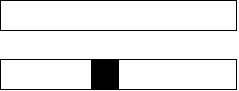
\includegraphics[scale=0.5]{figures/TTPProfiles/initImpl.pdf}} & I need your & \tabitem Shift H's attention & \tabitem Desire to start \\
               	& & full attention & towards T & a conversation \\
				& & & & \\
				\hline
               	\rule{0pt}{4ex}
               	\textbf{FLOOR\_TAKING\_RAW} & \multirow{3}{*}{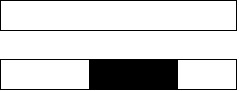
\includegraphics[scale=0.5]{figures/TTPProfiles/initRaw.pdf}} & I need your & \tabitem Shift H's attention & \tabitem Desire to start \\
           		& & full attention & towards T & a conversation \\
                & & & & \\                                                  
              	\hline
               	\rule{0pt}{4ex}
               	\textbf{FLOOR\_TAKING\_INTERP} & \multirow{3}{*}{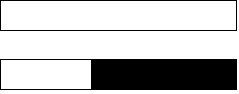
\includegraphics[scale=0.5]{figures/TTPProfiles/init.pdf}} & I need your & \tabitem Shift H's attention & \tabitem Desire to start \\
             	& & full attention & towards T & a conversation \\
               	& & because of x & & \tabitem More efficiency \\
        		& & & & by providing\\
                & & & & a justification\\
               	\hline
               	\rule{0pt}{4ex}
              	\textbf{DIALOGUE\_INIT} & \multirow{6}{*}{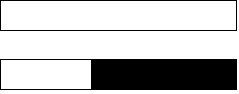
\includegraphics[scale=0.5]{figures/TTPProfiles/init.pdf}} & I start this & \tabitem Shift H's attention & \tabitem Desire to start \\
              	& & conversation and I & towards T & a conversation \\
               	& & inform you that x & \tabitem Make H aware & about x \\
              	& & & of the dialogue & \\
              	& & & topic (x) & \\
				& & & & \\
               	\hline
               	\rule{0pt}{4ex}
               	\textbf{FAIL\_IMPL} & \multirow{4}{*}{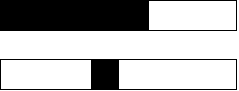
\includegraphics[scale=0.5]{figures/TTPProfiles/implBargeIn.pdf}} & I don't understand & \tabitem Make H stop & \tabitem Fix desynchro- \\
              	& & what you are & \tabitem Make H repeat & nisation \\
              	& & talking about & or reformulate & \\
				& & & & \\
               	\hline
              	\rule{0pt}{4ex}
               	\textbf{FAIL\_RAW} & \multirow{4}{*}{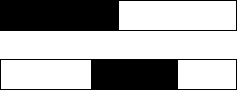
\includegraphics[scale=0.5]{figures/TTPProfiles/shortBargeIn.pdf}} & I don't understand & \tabitem Make H stop & \tabitem Fix desynchro- \\
             	& & what you are & \tabitem Make H repeat & nisation \\
           		& & talking about & or reformulate & \\
				& & & & \\
              	\hline
              	\rule{0pt}{4ex}
              	\textbf{FAIL\_INTERP} & \multirow{8}{*}{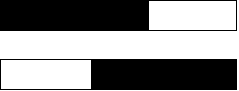
\includegraphics[scale=0.5]{figures/TTPProfiles/longBargeIn.pdf}} & I don't understand & \tabitem Make H stop & \tabitem Fix desynchro- \\
              	& & what you are & \tabitem Make H repeat & nisation \\
             	& & talking about & or reformulate & \\
             	& & because of x & \tabitem Making H aware & \tabitem More efficiency by \\
             	& & & of what is & providing more \\
               	& & & preventing T & precision about \\
              	& & & from understanding & the problem \\
				& & & & \\
               	\hline
                \rule{0pt}{4ex}
              	\textbf{FAIL\_MOVE} & \multirow{8}{*}{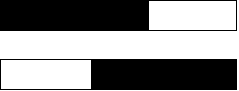
\includegraphics[scale=0.5]{figures/TTPProfiles/longBargeIn.pdf}} & I don't understand & \tabitem Make H stop & \tabitem Fix desynchro- \\
              	& & what you are & \tabitem Shift H's focus & nisation \\
             	& & talking about, & conversation & \\
             	& & consider x & towards x & \tabitem Moving the \\
             	& & instead & & conversation \\
               	& & & & forward \\
              	& & & & \\
				& & & & \\
               	\hline
               	\rule{0pt}{4ex}
          		\textbf{INCOHERENCE\_IMPL} & \multirow{5}{*}{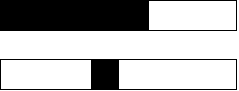
\includegraphics[scale=0.5]{figures/TTPProfiles/implBargeIn.pdf}} & What you just said & \tabitem Make H stop & \tabitem Fix desynchro- \\
             	& & is problematic & \tabitem Make H reconsider & nisation \\
            	& & & what he & \\
               	& & & just said & \\
				& & & & \\
               	\hline
              	\rule{0pt}{4ex}
              	\textbf{INCOHERENCE\_RAW} & \multirow{5}{*}{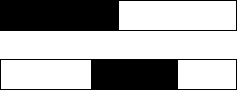
\includegraphics[scale=0.5]{figures/TTPProfiles/shortBargeIn.pdf}} & What you just said & \tabitem Make H stop & \tabitem Fix desynchro- \\
          		& & is problematic & \tabitem Make H reconsider & nisation \\
        		& & & what he & \\
            	& & & just said & \\
				& & & & \\
               	\hline
        	\end{tabular}
		}
        \caption{Taxonomy labels (1/3)}
        \label{tab:taxosynth}
  	\end{table}

  	\begin{table}[htp]
		\fontsize{8.2}{8.2}
        \selectfont
        \vspace{2mm}
        \centerline{
        	\begin{tabular}{|c|c|c|c|c|}
                \hline
                \textbf{TTP} & \textbf{Phonetic act} & \textbf{Illocutionary act} & \textbf{Perlocutionary act} & \textbf{Motivations} \\
                \hline
                \rule{0pt}{4ex} 
              	\textbf{INCOHERENCE\_INTERP} & \multirow{8}{*}{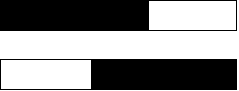
\includegraphics[scale=0.5]{figures/TTPProfiles/longBargeIn.pdf}} & What you just said & \tabitem Make H stop & \tabitem Fix desynchro- \\
              	& & is problematic & \tabitem Make H reconsider & nisation \\
               	& & because of x & what he & \tabitem More efficiency by \\
            	& & & just said & providing more \\
           		& & & \tabitem Making H aware & precision about \\
              	& & & of the problem & the problem \\
              	& & & in his utterance & \\
				& & & & \\
               	\hline
                \rule{0pt}{4ex} 
              	\textbf{INCOHERENCE\_MOVE} & \multirow{8}{*}{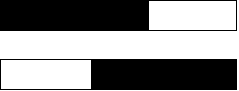
\includegraphics[scale=0.5]{figures/TTPProfiles/longBargeIn.pdf}} & What you just said & \tabitem Make H stop & \tabitem Fix desynchro- \\
              	& & is problematic & \tabitem Make H reconsider & nisation \\
               	& & because of x, & what he & \tabitem More efficiency by \\
            	& & consider y & just said & providing more \\
           		& & instead & \tabitem Making H aware & precision about \\
              	& & & of the problem & the problem \\
              	& & & in his utterance & \tabitem Moving the \\
				& & & \tabitem Shift H's focus & conversation \\
                & & & towards y & forward \\
                & & & & \\
               	\hline
                \rule{0pt}{4ex}
                \textbf{BACKCHANNEL} & \multirow{3}{*}{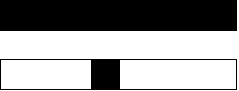
\includegraphics[scale=0.5]{figures/TTPProfiles/backchannel.pdf}} & I understand (and & \tabitem Make H continue & \tabitem More information \\
                & & sometimes: I agree) & & from H \\
                & & & & \\
                \hline
                \rule{0pt}{4ex}
                \textbf{FEEDBACK\_RAW} & \multirow{7}{*}{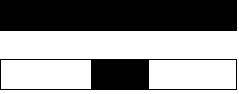
\includegraphics[scale=0.5]{figures/TTPProfiles/shortFb.pdf}} & I understood that & \tabitem Make H continue & \tabitem More information \\
                & & you said x & \tabitem Make H correct & from H \\
                & & & in case of a & \tabitem Desire to confirm\\
                & & & misunderstanding & that H's utterance\\
                & & & or not & has been well \\
                & & & & understood \\
                & & & & \\
                \hline
                \rule{0pt}{4ex}
                \textbf{FEEDBACK\_INTERP} & \multirow{10}{*}{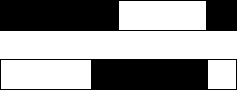
\includegraphics[scale=0.5]{figures/TTPProfiles/longFb.pdf}} & I understood that & \tabitem Make H continue & \tabitem More information \\
                & & you said x & \tabitem Make H correct & from H \\
                & & that is related  & in case of a & \tabitem Desire to confirm\\
                & & to y & misunderstanding & that H's utterance\\
                & & & or not & has been well \\
                & & & & understood \\
                & & & & \tabitem Stronger confirmation \\
                & & & & by adding related \\
                & & & & information y \\
                & & & & \\
                \hline
                \rule{0pt}{4ex}
                \textbf{BARGE\_IN\_CHANGE} & \multirow{10}{*}{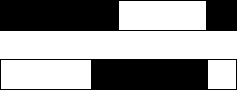
\includegraphics[scale=0.5]{figures/TTPProfiles/longFb.pdf}} & I understood that & \tabitem Shift H's focus & \tabitem More information \\
                & & you said x, & towards x & about x \\
                & & tell me more & & \\
                & & about it & & \\
                & & & & \\
                \hline
                \rule{0pt}{4ex}
                \textbf{REF\_IMPL} & \multirow{6}{*}{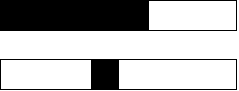
\includegraphics[scale=0.5]{figures/TTPProfiles/implBargeIn.pdf}} & Yes, x & \tabitem Make H stop & \tabitem Selecting an option\\
                & & & and understand & \tabitem Less effort as x \\
                & & & T is referring to & has already been \\
                & & & the last element & uttered by H \\
                & & & he uttered (x) & \\
                & & & & \\
                \hline
       		\end{tabular}
       	}
        \caption{Taxonomy labels (2/3)}
        \label{tab:taxosynth2}
	\end{table}
    
    \begin{table}[htp]
		\fontsize{8.2}{8.2}
        \selectfont
        \vspace{2mm}
        \centerline{
        	\begin{tabular}{|c|c|c|c|c|}
                \hline
                \textbf{TTP} & \textbf{Phonetic act} & \textbf{Illocutionary act} & \textbf{Perlocutionary act} & \textbf{Motivations} \\
                \hline
                \rule{0pt}{4ex}
                \textbf{REF\_RAW} & \multirow{9}{*}{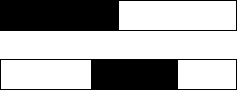
\includegraphics[scale=0.5]{figures/TTPProfiles/shortBargeIn.pdf}} & Yes, x & \tabitem Make H stop & \tabitem Selecting an option\\
                & & & and understand & \tabitem Less effort as x \\
                & & & T is referring to & has already been \\
                & & & the last element & uttered by H \\
                & & & he uttered (x) & \tabitem Desire to confirm \\
                & & & \tabitem Make H correct & that the last option \\
                & & & in case of a & has been well \\
                & & & misunderstanding & understood \\
                & & & & \\
                \hline
                \rule{0pt}{4ex}
                \textbf{REF\_INTERP} & \multirow{12}{*}{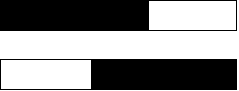
\includegraphics[scale=0.5]{figures/TTPProfiles/longBargeIn.pdf}} & Yes, x that & \tabitem Make H stop & \tabitem Selecting an option\\
                & & is related to y & and understand & \tabitem Less effort as x \\
                & & & T is referring to & has already been \\
                & & & the last element & uttered by H \\
                & & & he uttered (x) & \tabitem Desire to confirm \\
                & & & \tabitem Make H correct & that the last option \\
                & & & in case of a & has been well \\
                & & & misunderstanding & understood \\
                & & & & \tabitem Stronger confirmation \\
                & & & & by adding related \\
                & & & & information y \\
                & & & & \\
                \hline
                \rule{0pt}{4ex}
                \textbf{BARGE\_IN\_RESP} & \multirow{10}{*}{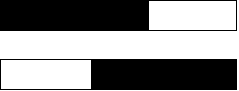
\includegraphics[scale=0.5]{figures/TTPProfiles/longBargeIn.pdf}} & x & \tabitem Make H aware & \tabitem Desire to move \\
                & & & of x & the dialogue \\
                & & & & forward \\
                & & & & \tabitem More efficiency \\
                & & & & because enough \\
                & & & & information has \\
                & & & & been provided before \\
                & & & & the end of the \\
                & & & & utterance \\
                & & & & \\
                \hline
                \rule{0pt}{4ex}
                \textbf{REKINDLE\_IMPL} & \multirow{6}{*}{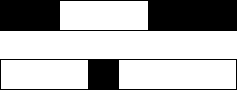
\includegraphics[scale=0.5]{figures/TTPProfiles/rekindle.pdf}} & The information you & \tabitem Make H resume & \tabitem Fix desynchronisation \\
                & & gave is not & & \\
                & & enough, please & & \\
                & & provide more & & \\
                & & information & & \\
                & & & & \\
                \hline
                \rule{0pt}{4ex}
                \textbf{REKINDLE\_RAW} & \multirow{6}{*}{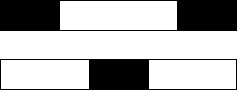
\includegraphics[scale=0.5]{figures/TTPProfiles/rekindleRaw.pdf}} & The information you & \tabitem Make H resume & \tabitem Fix desynchronisation \\
                & & gave is not & & \\
                & & enough, please & & \\
                & & provide more & & \\
                & & information & & \\
                & & & & \\
                \hline
                \rule{0pt}{4ex}
                \textbf{REKINDLE\_INTERP} & \multirow{6}{*}{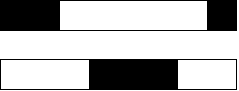
\includegraphics[scale=0.5]{figures/TTPProfiles/rekindleInterp.pdf}} & The information you & \tabitem Make H provide & \tabitem Complete \\
                & & gave is not & information x & understanding \\
                & & enough, please & & of H's \\
                & & provide & & utterance \\
                & & information x & & \\
                & & & & \\
                \hline
                \rule{0pt}{4ex}
                \textbf{END\_POINT} & \multirow{4}{*}{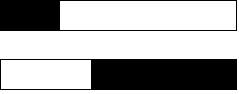
\includegraphics[scale=0.5]{figures/TTPProfiles/endPoint.pdf}} & x & \tabitem Make H aware & \tabitem Desire to move \\
                & & & of x & the dialogue \\
                & & & & forward \\
                & & & & \\
                \hline
       		\end{tabular}
       	}
        \caption{Taxonomy labels (3/3)}
        \label{tab:taxosynth3}
	\end{table}
		
	 \section{Turn-taking phenomena in dialogue systems}
	
				INIT\_DIALOGUE is a TTP that is involved in every dialogue system, including traditional ones. FLOOR\_TAKING TTPs are of limited interest when it comes to task-oriented dialogue, therefore, they are not implemented in task-oriented dialogue systems. There are two ways of initialising the dialogue, the user initiative one (the user starts speaking first like this is the case for Siri for instance) and the system initiative way (the system delivers an initial prompt, when calling an IVR for example). END\_POINT is also necessary for any kind of dialogue, however, the way the dialogue participants exchange turns is not always the same given the situation at hand. Humans are very good at detecting end of utterance clues beforehand, making T able to anticipate the right moment to take the floor hence achieving smooth turn-taking. Traditional dialogue systems, on the other hand, rely on long enough silences as markers of end of turn. A research thread is dedicated to studying methods of reducing these silences by considering different clues (prosodic, lexical and semantic) aiming for smoother turn exchange \cite{Raux2008,Gravano2011}. However, even though they have been under study for many years, there is still room for improvement. In the rest of this section, the remaining TTPs are discussed (that can be replicated in incremental dialogue systems only) from an implementation point of view. Our goal is to come up with a list of TTPs that are the most likely to improve task-oriented dialogue. Similarly, the REKINDLE TTPs correspond to dialogue management strategies that can be implemented in any traditional dialogue system and as a consequence, it will not be considered here. Moreover, since this thesis focuses on task oriented dialogue, FAIL\_MOVE, INCOHERENCE\_MOVE and BARGE\_IN\_CHANGE are not discussed neither since they are aimed to change the discussion topic.

				Before leading this discussion, it is important to notice that each TTP has two symmetric versions when it comes to human-machine dialogue: the one where H is the user and T is the machine and the opposite case. Here, the goal is to study system decisions therefore only one side is mainly studied (even though a TTP is implemented from both sides). In order for both cases to be implemented, the incremental dialogue system at hand should always be listening to the user, even though it has the floor (hence being able to be interrupted). As a technical side note, current incremental dialogue systems are used with a headphone for that reason: as the system keeps listening all the time, it is a convenient way to prevent it from hearing itself while speaking (considering its own sentence as a user input). In order to make them useful outside of labs, in more realistic situations, it is necessary to build algorithms that suppress the TTS result from the ASR input before feeding it to the latter (which raises a new challenge as it must also be done incrementally). Moreover, in this thesis, the focus is on the vocal modality. Therefore, no TTP based on gestures is considered for implementation.

				Implementing a mechanism that mimics the FAILn TTPs is an interesting idea to explore. Users frequently use off-domain words and expression \cite{Ghigi2014} and they are also ofter misunderstood by the ASR. As a consequence, making the system barge-in when it does not understand the user's partial utterance might have a positive impact on the dialogue efficiency. It might be less tiresome for the user as she wouldn't have to repeat her whole sentence several times. Moreover, this reduces the dialogue duration. FAIL\_RAW is not easy to replicate by a machine and it is most of the time performed with gestures and facial expressions at the same time. FAIL\_INTERP is not easy to implement neither as giving the accurate reason why it did not manage to understand the user's utterance so far is not an obvious task. Implementing FAIL\_RAW, on the other hand, is much more realistic: when the systems has no clue about the user's utterance after a long enough period of time, it simply declares that fact in a straightforward fashion.

				In some cases, the user is likely to utter a sentence that is not coherent for the system or that is in contradiction with some data accessible by the latter (like when trying to buy a movie ticket when all the seats are already sold). By definition, the INCOHERENCE TTPs can help manage this case in a more efficient way. For the same reasons as FAIL\_RAW, INCOHERENCE\_RAW is not easy to implement. Unlike FAIL TTPs, it is not natural and more difficult to declare an incoherence without explaining the underlying reasons. Therefore, INCOHERENCE\_INTERP is the most interesting TTP to implement.

				BACKCHANNEL has already been implemented in a few incremental dialogue systems \cite{Meena2013,Hastie2013} with the aim of increasing its grounding capacities and its naturalness. This thesis focuses more on the efficiency aspect of incremental dialogue than the human-likeness side of the problem. These are somehow correlated, but as this is not a TTP that directly makes the dialogue more efficient (by preventing and fixing errors), it will not be implemented. Moreover, as the first step of the approach followed here is to use simulated dialogues, it is hard to evaluate this TTP in such conditions. On the contrary, FEEDBACK\_RAW provides a concrete opportunity to correct errors. When T tries to repeat a part of H's utterance and she succeeds, this gives H a proof that T heard his sentence (even though, this does not necessarily mean that T has well understood the message). If she fails, it is also interesting as H can repeat or reformulate his utterance, hence avoiding a desynchronisation. This is clearly interesting to be implemented in a dialogue system, yet, it can be very challenging. The involved turn-taking mechanism is difficult to manage in the sense that the user should not interpret the system's intervention as a barge-in hence being interrupted. Moreover, the system should be able to recognise whether the user ignored the feedback or tried to correct its content. Therefore, this TTP has been implemented in simulation only. Finally, FEEDBACK\_INTERP requires high NLP capabilities and access to an important knowledge base. Therefore, it has not been implemented here.

				In \cite{El-Asri2014a}, REF\_RAW has been implemented from the user's point of view: the system enumerates a list of alternatives and the user barges-in to select one of them. This has been shown to significantly increase the dialogue quality \cite{El-Asri2014c}. However, implementing it requires changing the dialogue management strategy whereas, as discussed in Chapter \ref{ch:architecture}, this thesis focuses on the impact of adding a turn-taking layer on top of pre-existing dialogue management strategies. As a consequence, REF\_IMPL, REF\_RAW and REF\_INTERP are not studied here.

				Finally, BARGE\_IN\_RESP is clearly worth implementing from both sides. From the system's perspective, taking the floor as soon as it has enough information to do so can directly increase dialogue efficiency by reducing dialogue duration but also indirectly by preventing the user from adding new misleading information \cite{Ghigi2014}. From the user's point of view, being able to take the floor before the end of the system's utterance can make the dialogue less tiresome. This is especially true for users that are familiar with the system and as a consequence, they are able to predict the rest of the systems dialogue acts ahead of time.

				To summarise, four TTP requiring incremental dialogue processing have been selected for rule-based implementation (one of them from both sides: system and user):
				\begin{itemize}
					\item FAIL\_RAW (System side\footnote{\textit{System side} means that the turn-taking decision is made by the system. In other words, T is the system. \textit{User side} designates the opposite situation.})
					\item INCOHERENCE\_INTEPR (System side)
					\item FEEDBACK\_RAW (System side)
					\item BARGE\_IN\_RESP (System and user side)
				\end{itemize}

				In Chapter \ref{ch:baseline}, the details of the implementation, the rules chosen as well as a comparative study in a simulated environment are provided.
